\documentclass[a4paper]{article}
\usepackage[italian]{babel}
\usepackage{booktabs}
\usepackage{siunitx}%Questo serve a caricare il pacchetto delle unità di misura del sistema internazionale%
\usepackage[utf8]{inputenc}
\usepackage{graphicx} 
\usepackage{url}
\usepackage{amsmath}
\usepackage{amssymb}
\usepackage{listings}
\usepackage{multirow}
\usepackage{textcomp,marvosym}
\usepackage{keyval}
\usepackage{xcolor}
\usepackage{caption}
\usepackage{subcaption}
\usepackage{subfig}
\usepackage{tikz}
\usepackage{circuitikz}
\usepackage{authblk}
%\usepackage{hyperref}
\lstset{language=C}
\lstset{basicstyle=\small\ttfamily,
keywordstyle=\color{black}\bfseries,
commentstyle=\color{darkgray},
stringstyle=\color{black},
showstringspaces=true}

\begin{document}

\title{Tecnologie Digitali - Relazione di laboratorio: I-V remoto}
	\author[1]{Salvatore Bottaro}
		\author[2]{Lorenzo M. Perrone}
		\affil[1]{\texttt{salvo.bottaro@hotmail.it}}
		\affil[2]{\texttt{lorenzo.perrone.lmp@gmail.com}}
	\markboth{Tecnologie Digitali - Di Lieto}{}
	\maketitle

\section{Modello di Shockley}
La prima domanda che ci poniamo è se il modello esponenziale di Shockley per le giunzioni a semiconduttore riesca a spiegare bene i dati che abbiamo acquisito o se invece vi sono deviazioni significative da esso. Il modello nella sua espressione più semplice prevede una relazione fra I e V come segue:

\begin{equation}
I = A \left( exp(BV)-1 \right)
\end{equation}

dove $B = e/nKT$. Una forma meno rozza prevede la presenza di un ulteriore parametro additivo $C$ che fisicamente rappresenta la \textit{bias current}.

\begin{equation}
I = A \left( exp(BV)-1 \right) + C
\end{equation}

Consideriamo la temperatura (effettiva) di 46.6 °C e proviamo dunque a fittare entrambi i modelli appena riportati. Utilizziamo un range di correnti in cui non si arriva a valori troppo elevati, vale a dire 1-120 $\mu$A, circa, in cui siano visibili gli effetti di tutti i termini dell'equazione di Shockley. Gli errori sulle correnti sono stati posti pari a $\sigma_I = 0.05 \mu$A, (due-tre volte maggiore della sensibilità nominale della strumentazione), quelli sulle tensioni pari a $\sigma_V = 0.3$mV.\\
Per il fit di Shockley-2 (a due parametri), i risultati ottenuti sono:

\begin{table}[h]
\centering
\begin{tabular}{c|c|l}
 \textbf{A} [$\mu$A] & \textbf{B} [$V^{-1}$] & $\chi_{rid}^2$\\ 
\hline 0.01359(10) & 19.49(1) & 5.5 \\ 
\end{tabular} 
\end{table}
~\\

Per il fit di Shockley-3 abbiamo invece:

\begin{table}[h]
\centering
\begin{tabular}{c|c|l|l}
 \textbf{A} [$\mu$A] & \textbf{B} [$V^{-1}$] & \textbf{C} [$\mu$A]  & $\chi_{rid}^2$\\ 
\hline 0.01314(11) & 19.56(2) & 0.18(4) & 5 \\
\end{tabular} 
\end{table}
~\\

Nelle Figure (\ref{fig:shockley_3_pars_46gradi_semilogy},\ref{fig:shockley_3_pars_46gradi}) è riportato sia in scala semilogy che lineare il fit di Shockley-3, visualizzando solo le correnti nel range di interesse 1-120 $\mu$A. Nel grafico in scala lineare non si evidenziano dei sostanziali scostamenti dalla curva di fit dei dati sperimentali per correnti inferiori alla decina di $\mu$ A, che invece sono ben visibili in scala semilog.\\

\begin{figure}
\centering
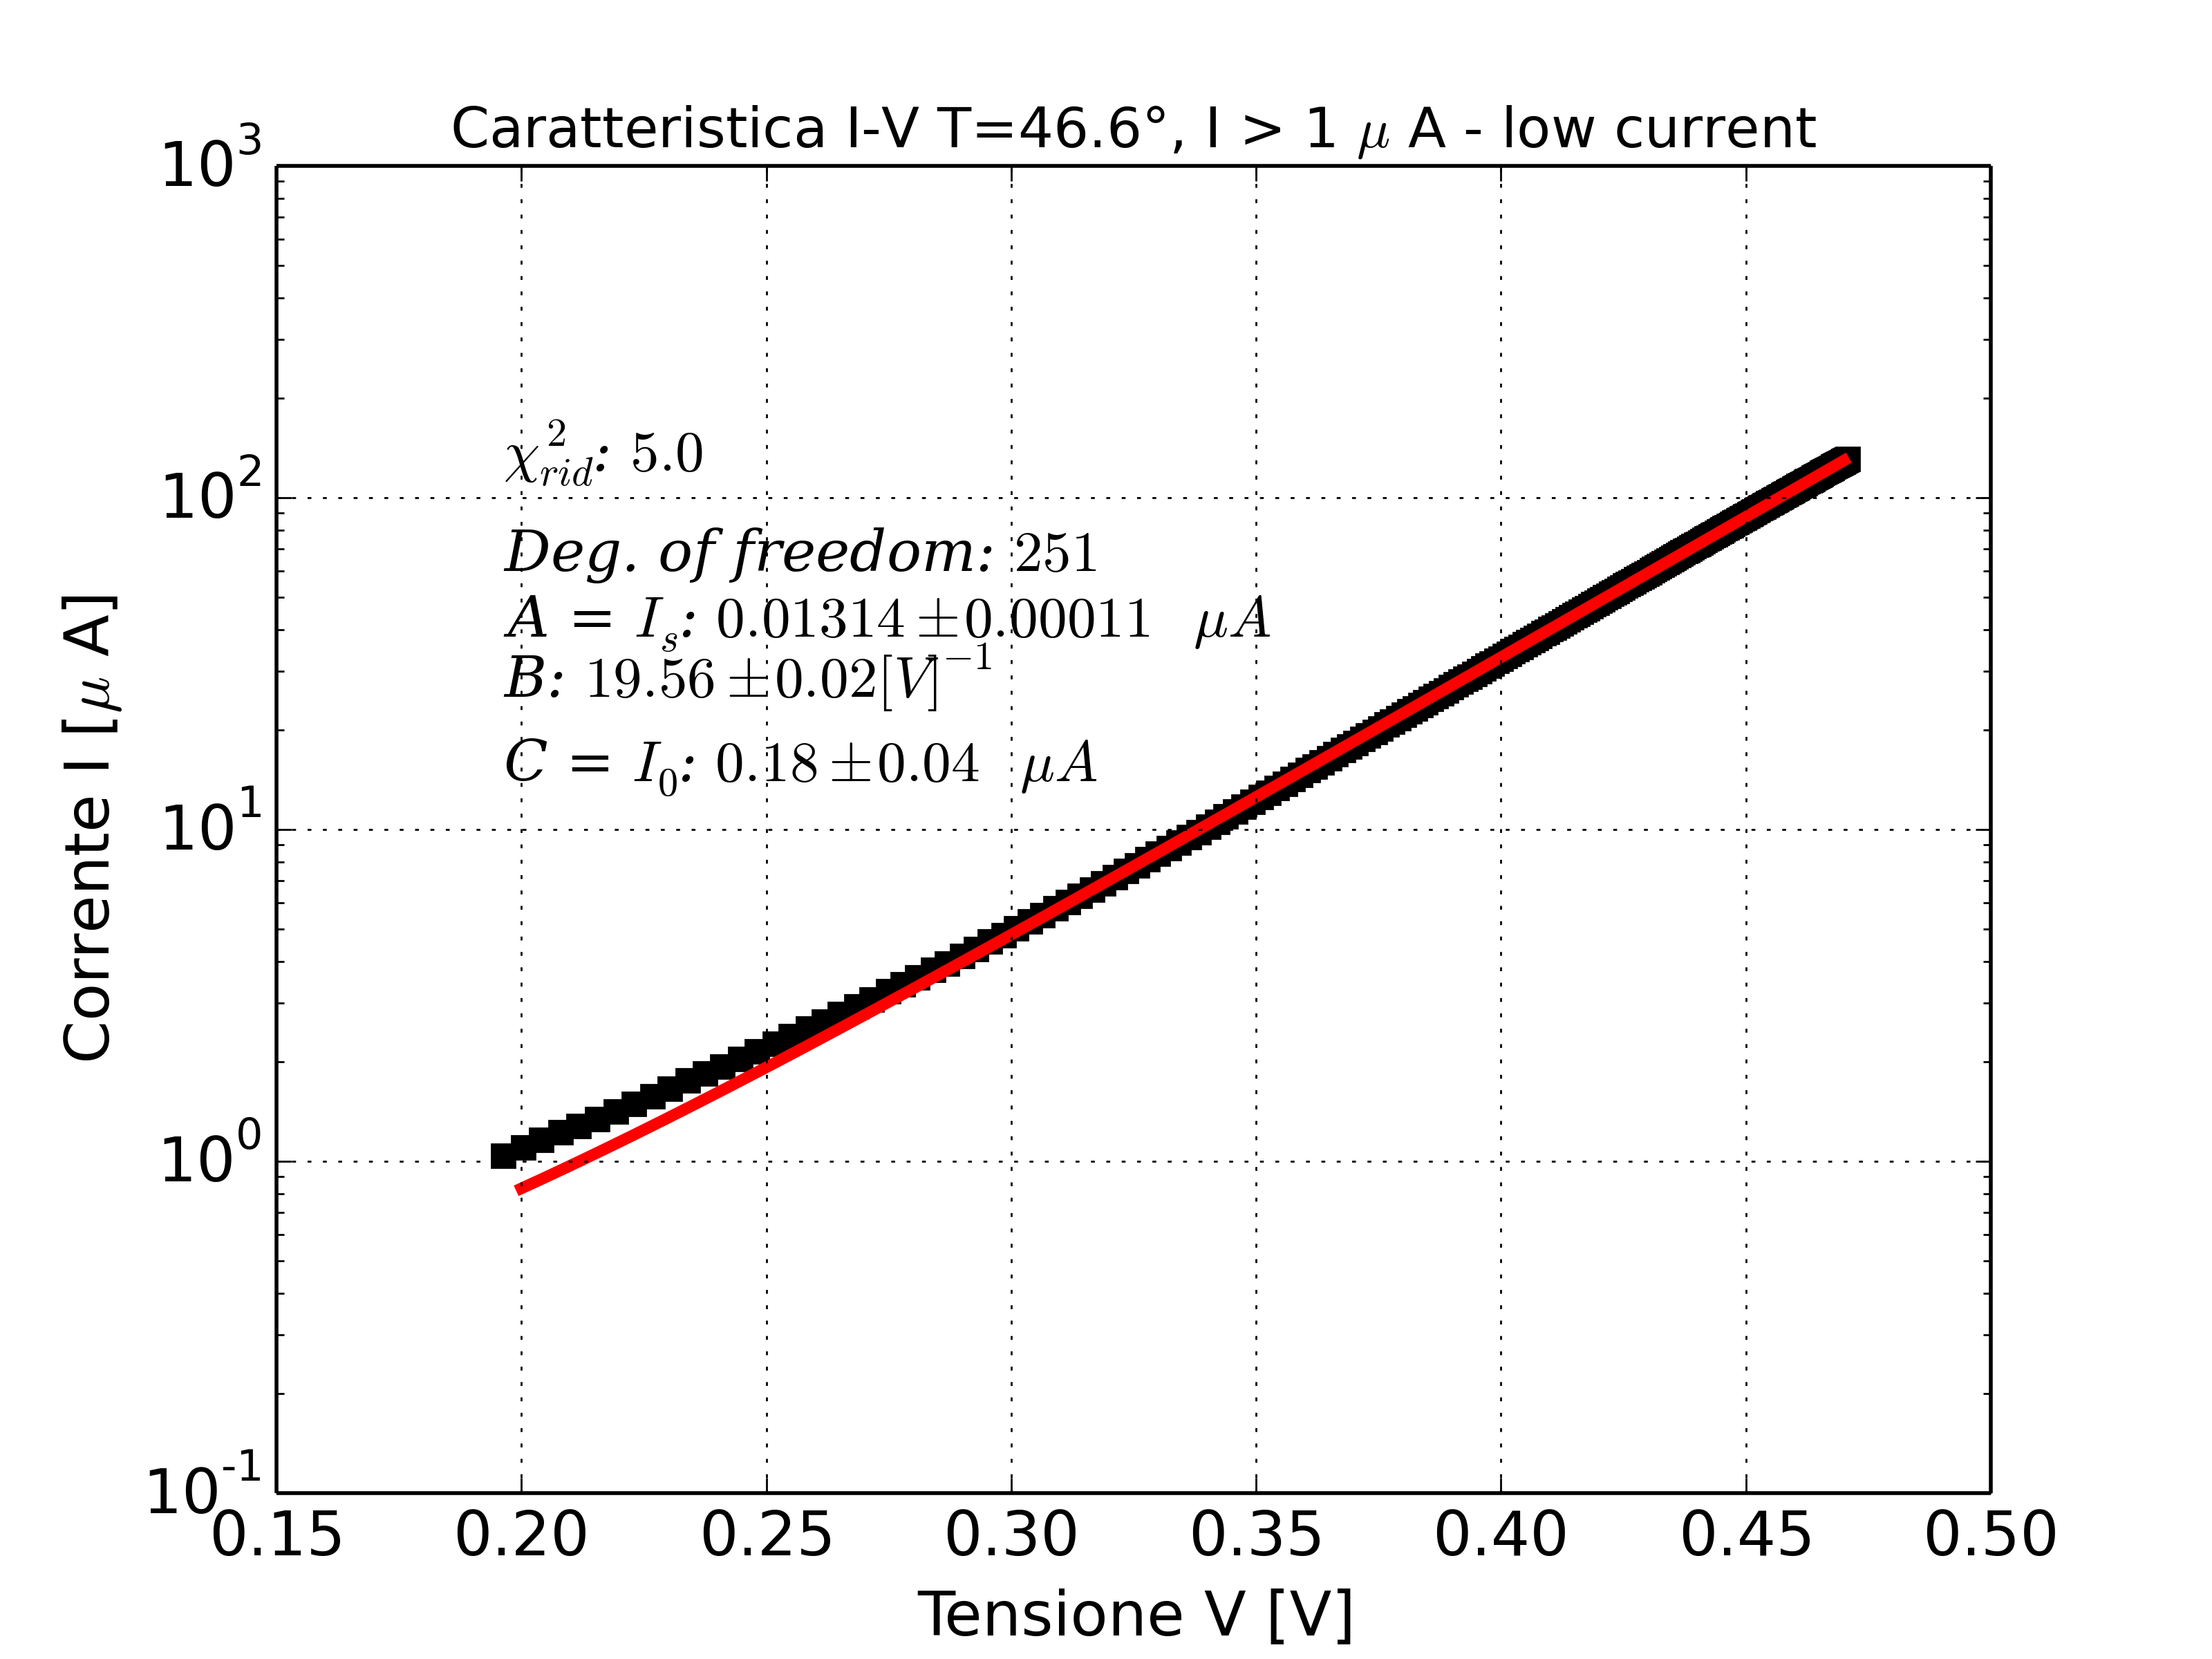
\includegraphics[width=0.9\linewidth]{./shockley_3_pars_46gradi_semilogy}
\caption{Fit di Shockley-3 semilogy: correnti nel range 1-120 $\mu$A}
\label{fig:shockley_3_pars_46gradi_semilogy}
\end{figure}

\begin{figure}
\centering
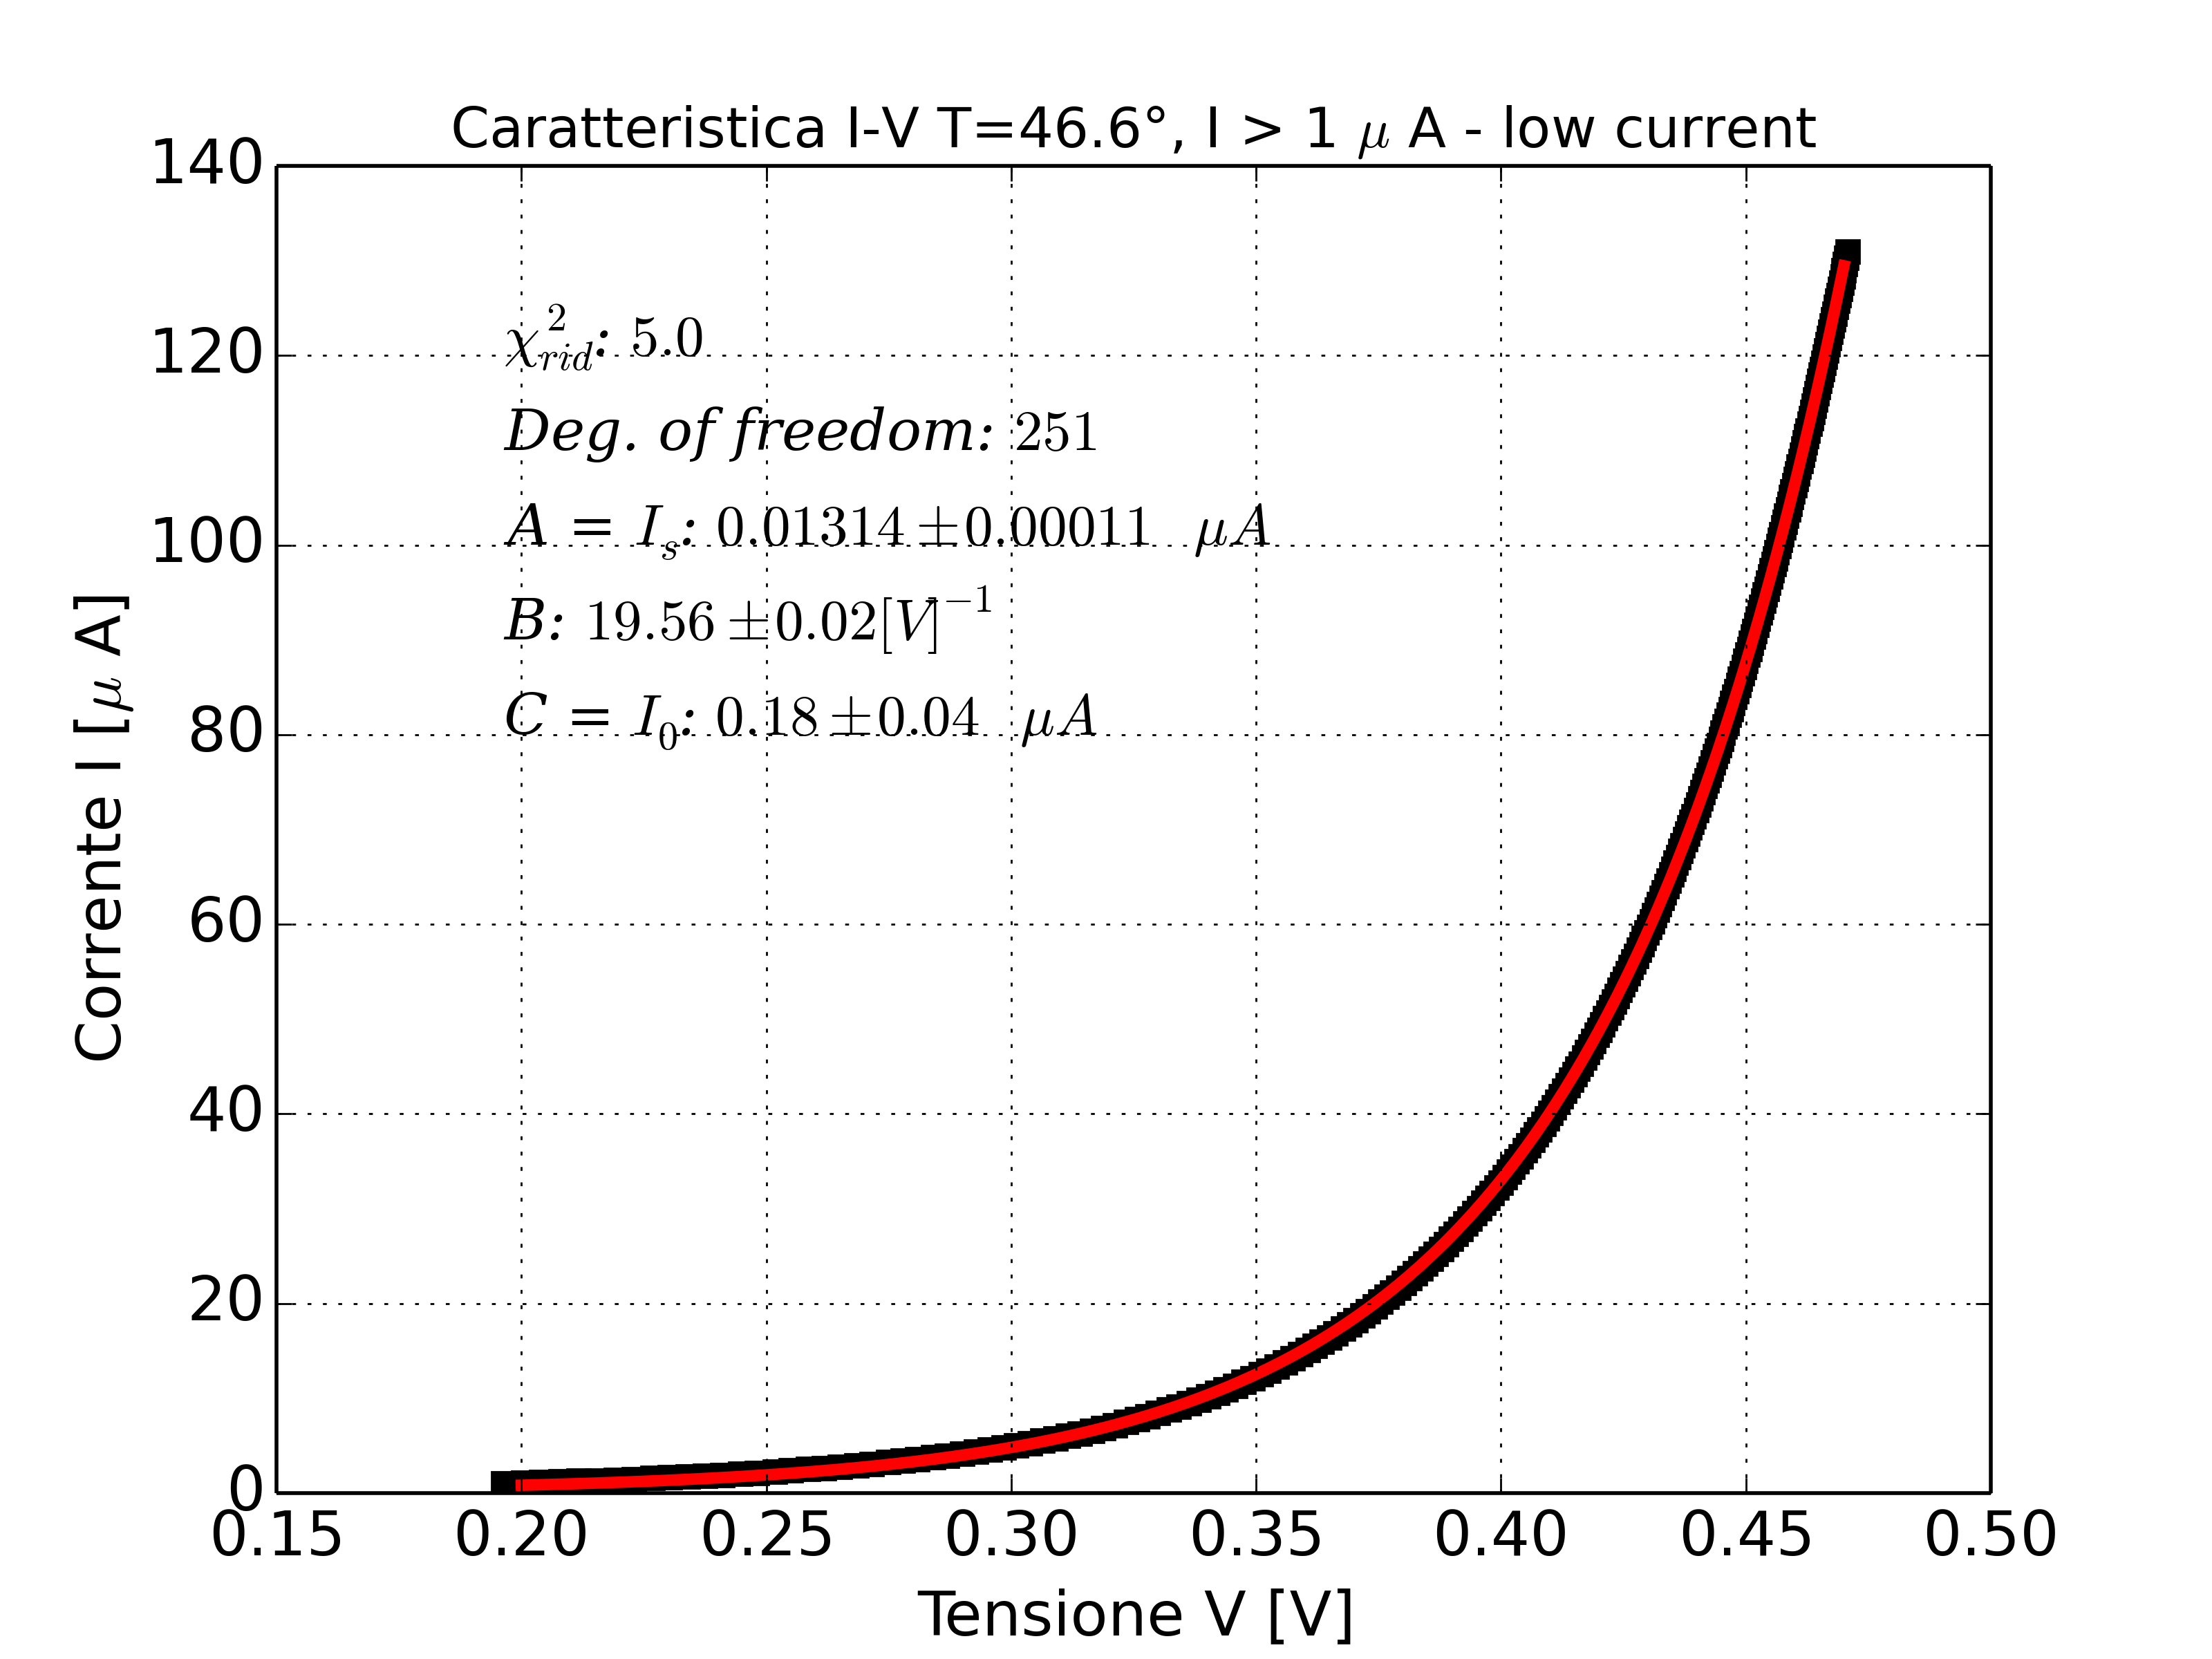
\includegraphics[width=0.9\linewidth]{./shockley_3_pars_46gradi}
\caption{Fit di Shockley-3 lineare: correnti nel range 1-120 $\mu$A}
\label{fig:shockley_3_pars_46gradi}
\end{figure}

Plottiamo ora le stesse funzioni di fit, sovrapponendole però al range completo delle correnti a nostra disposizione per verificare la validità del modello in uso su una più larga scala. Nello stesso grafico di Figura (\ref{fig:shockley_46_6_fullcur_visualiz}) sono riportate (con colori diversi) entrambe le curve di Shockley.

\begin{figure}
\centering
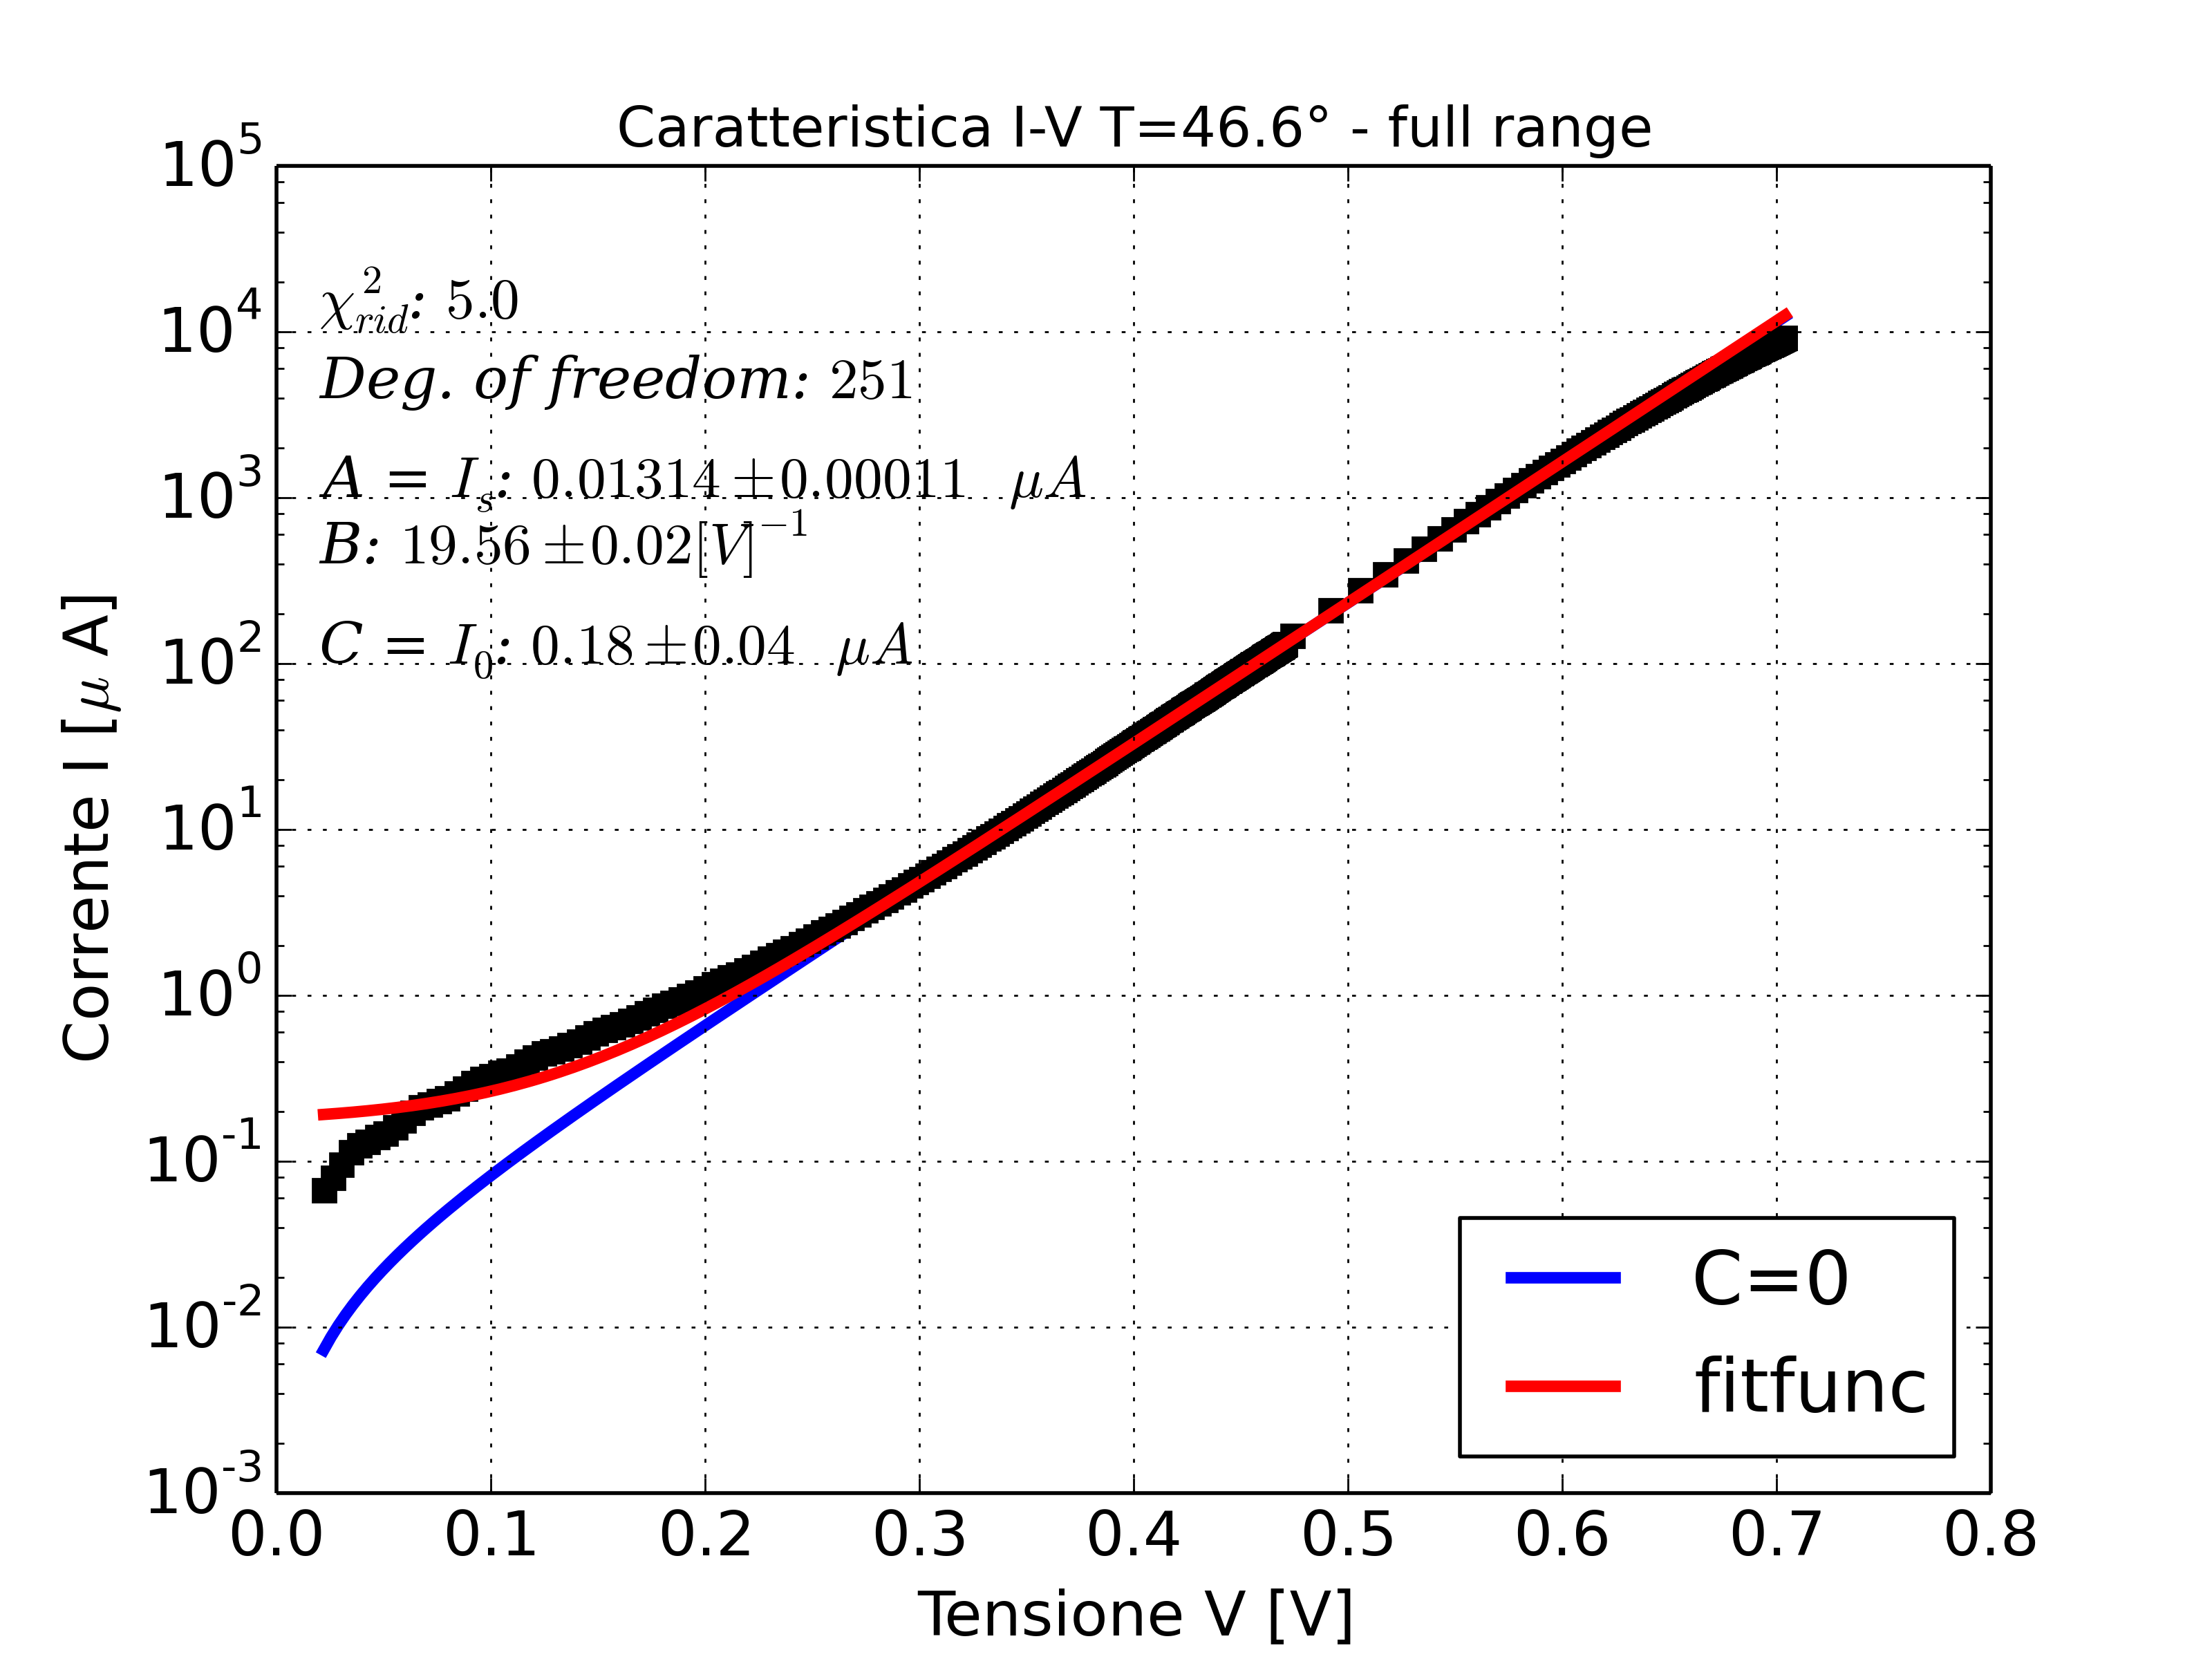
\includegraphics[width=0.9\linewidth]{./shockley_46_6_fullcur_visualiz}
\caption{Curve di fit Shockley-2 e Shockley-3 sovrapposte all'intero range di correnti.}
\label{fig:shockley_46_6_fullcur_visualiz}
\end{figure}


\section{Deviazioni dal modello di Shockley}

Come è evidente dal fit riportato in Figura (\ref{fig:shockley_3_pars_46gradi_semilogy}) e relativo ad un range di correnti 0.1-100 $\mu$A, il modello esponenziale di Shockley produce un buon accordo con i dati sperimentali solo per correnti dell'ordine di decine di $\mu$A: per valori più bassi, il fit di Shockley a due parametri sottostima anche di un ordine di grandezza $I$, mentre per correnti maggiori di $10^3-10^4 \mu$A queste sono sovrastimate (vedi Figura (\ref{fig:shockley_46_6_fullcur_visualiz})).\\
I fenomeni che possono spiegare questi comportamenti sono essenzialmente due. Ad alte correnti potrebbero iniziare ad essere rilevanti dei comportamenti ohmici della struttura che ospita la giunzione, per cui, a parità di fem, la differenza di potenziale applicata ai capi di quest'ultima è inferiore (quindi correnti inferiori). In regime di basse correnti, invece, possiamo supporre che si evidenzi come un collegamento in parallelo rispetto al diodo, attraverso il quale scorre una quantità di carica paragonabile a quella che passa nella giunzione.\\

Una modellizzazione che tenga conto di questi due fenomeni è la seguente:

\begin{equation}\label{corrente_totale}
I = I_p + I_J = GV + I_S \left[exp(B(V-R_s I_J)-1))\right]
\end{equation}

e il corrispettivo schema circuitale è in Figura (\ref{fig:schema_circuit}).\\

\begin{figure}
\centering
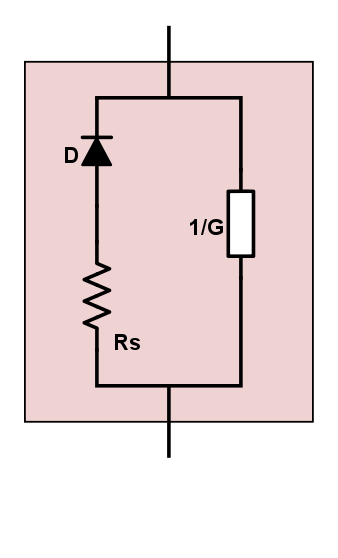
\includegraphics[width=0.3\linewidth]{./schema_circuit}
\caption{Schema circuitale del modello "reale" presentato}
\label{fig:schema_circuit}
\end{figure}


Con $G$ indichiamo il reciproco della resistenza parallela equivalente, con $I_J$ la corrente che scorre nella giunzione, $R_s$ è la resistenza in serie alla giunzione stessa. Un buon fit dei dati dovrà, quindi, tenere conto contemporaneamente dell'influenza del ramo in parallelo, visibile a basse correnti, e della resistenza in serie, che si evidenzia ad alte $I$.\\

Un modo per considerare allo stesso tempo questi due fattori è quello di ricorrere ad una procedura iterativa su tutti i dati di corrente e che, ottimisticamente, converga a dei valori accettabili dei parametri $G$, $R_s$, $I_S$, $B$.

\section{Procedura iterativa di fit}
La procedura iterativa si basa, essenzialmente, su di una serie di passaggi che di volta in volta migliorano le stime dei parametri ottenuti nei passi precedenti. In particolare:

\begin{enumerate}

\item Come prima stima del parametro G, implementiamo un fit lineare sui dati a basse correnti ($I \lesssim 1 \mu$A) del tipo $I = GV$. Si rimanda alla sezione () per alcune annotazioni su questo passo.

\begin{lstlisting}
g_0, pcov_lin = optimize.curve_fit(linfit, 
xdata[:argmax(ydata>=1)], ydata[:argmax(ydata>=1S)], p0lin, sigmay)
\end{lstlisting}

\item INIZIO LOOP: Con la stima di $G^{i=0}$ possiamo ottenere un primo valore della corrente che scorre nella giunzione $I_J = I - G^i V$.

\begin{lstlisting}
jun_cur = ydata - g_0*xdata
\end{lstlisting}

\item Per regimi di correnti non troppo alti, il primo termine nella (\ref{corrente_totale}) è trascurabile rispetto al comportamento esponenziale. La relazione si può dunque riscrivere come:

\begin{equation}
V(I=I_J) = \frac{1}{B} log \left(\frac{I}{I_J} + 1 \right) + R_s I
\end{equation}

Fittiamo ora questa funzione esplicita di $I_J$ per ottenere la prima stima dei tre parametri rimasti $I_S^i$, $R_s^i$, $B^i$.

\begin{lstlisting}
p_loop, pcov_loop = optimize.curve_fit(tension_junc, 
abs(jun_cur[argmax(jun_cur>=sup_current):]), 
xdata[argmax(jun_cur>=sup_current):], p0_loop, sigmax)
\end{lstlisting}


\item Avendo ottenuto i parametri $I_S^i$, $R_s^i$, $B^i$, possiamo impiegarli risolvendo a ritroso l'equazione precedente e trovare così i valori aggiornati della corrente di giunzione $I_{J}^{i+1}$. La risoluzione questa volta è numerica, dato che l'espressione in funzione di $I_J$ è in forma implicita, e per implementarla usiamo la routine \textsc{fsolve} di Python:

\begin{lstlisting}
def fitsolve(I_j, I_s, B, R, v):
    return v - log(abs(I_j)/abs(I_s) + 1)/B + I_j*R*10**(-6)
jun_cur_1 = optimize.fsolve(fitsolve, jun_cur, (I_S, B, R_s, xdata) );
\end{lstlisting}

\item A partire dal nuovo array $I_{J}^{i+1}$ calcoliamo $I^{i+1} = G^i V + I_{J}^{i+1}$

\begin{lstlisting}
tot_cur = g_0*xdata + jun_cur_1
\end{lstlisting}

\item Similmente al passo introduttivo al loop, volendo cercare una correzione al parametro $G^i$, possiamo fittare la differenza fra i dati sperimentali $I$ e $I^{i+1}$, con la funzione: $I - I^{i+1} = \delta G \; V$, e il nuovo valore $G^{i+1}$ sarà quindi dato da $G_{i+1} = G^i +\delta G$. Anche in questo caso, i valori di correnti che andremo a selezionare per il fit saranno solo quelle al di sotto della nostra soglia di 1$\mu$A.

\begin{lstlisting}
delta_g, delta_g_pcov = optimize.curve_fit(linfit, xdata[:argmax(tot_cur>=1)],
ydata[:argmax(tot_cur>=1)]-tot_cur[:argmax(tot_cur>=1)], g_0, sigmay);

g_1 = g_0 + delta_g
\end{lstlisting} 

\item FINE LOOP: come ultimo passo prima di chiudere il loop, è necessario confrontare i parametri (i+1) con quelli (i) e definire un qualche criterio di convergenza. Quello da noi individuato, in seguito a diversi tentativi, è verificare se:

\begin{equation}
\left| X^{i+1} - X^{i}  \right| < \frac{\delta X^{i+1}}{M}
\end{equation}

con $M$ un'opportuna costante positiva maggiore di 1. Se tale condizione viene verificata contemporaneamente per tutti e 4 i parametri in gioco, allora il ciclo loop si ferma.

\end{enumerate}

\subsection{Annotazioni sul fit iterativo}
E' opportuno chiarire meglio alcuni passaggi della procedura iterativa.\\

\begin{itemize}

\item Al passo 1 (introduttivo al ciclo loop) si è verificato che la stima prodotta di $G^0$ con il fit lineare del modello $I = GV$ sui primi valori di corrente dà una stima soddisfacente, (indicativamente diciamo $G \lesssim 6-7 \mu S$) tale per cui la convergenza del parametro G nel loop si verifica, solo per temperature non superiori ai 50-60 °C. Al di sopra di questo valore il risultato della stima di G non permette la convergenza, poichè ad ogni iterazione questo aumenta in maniera monotona. In questi casi, allora, è stato ritenuto opportuno usare un modello di fit che includa sia la parte lineare che quella esponenziale: procedendo in tale modo la convergenza si è sempre verificata.


\item Al passo 3 è stata posta una condizione aggiuntiva sul range dei dati su cui fittare i parametri, e cioè che vengano prese solo le correnti (di giunzione) superiori ad un certo valore, posto arbitrariamente a 10$\mu$A. Si è osservato, nel corso di prove successive, che la convergenza, e soprattutto la stima numerica dei parametri restituiti dal fit, sembra migliore. Possiamo giustificare questo comportamento ricordandoci che questa forma funzionale è tanto più valida quanto maggiori sono le correnti in gioco, per cui la usiamo in un range opportuno di correnti di giunzione.\\

\section{Determinazione dell'energy gap della giunzione}
\subsection{Determinazione a partire dai parametri in funzione di T}

Dai dati ottenuti è possibile ottenere, in più modi diversi, l'energy gap del diodo. Infatti la corrente di saturazione inversa è legata alla temperatura da una relazione del tipo:

\begin{equation}
I_S = AT^{\delta} \exp \Big (-\frac{E_G}{nkT} \Big)
\label{eqn:schock}
\end{equation}

dove \emph{A} dipende dalle caratteristiche della giunzione (geometria, drogaggio...), l'esponente $\delta$ dipende dal tipo di diodo e nel nostro caso vale $\delta = 1.5 - 2$ (per le giunzioni delle celle fotovoltaiche vale 3). In figura \ref{fig:iesse} è mostrato l'andamento della corrente di saturazione inversa in funzione dell'inverso della temperatura.

\begin{figure}[!h]
\centering
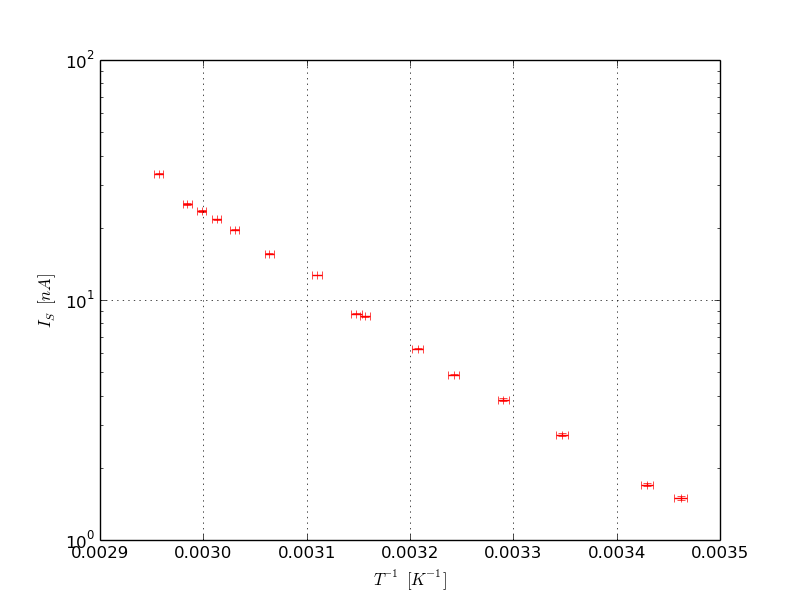
\includegraphics[scale=.5]{iesse}
\caption{$I_S$ in funzione dell'inverso della temperatura}
\label{fig:iesse}
\end{figure}

L'andamento esponenziale è dominante, il che suggerisce di trascurare in prima approssimazione il termine $T^{\delta}$ nell'equazione \ref{eqn:schock}. Il termine $\frac{1}{nkT}$ può essere inglobato nel coefficiente B ottenuto dal fit precedente. Nell'esecuzione del fit impegando direttamente la funzione \ref{eqn:schock} si è avuto un problema di overflow nel calcolo degli esponenziali, per cui è stato effettuato in due modi: il primo modo prendendo il logaritm di entrambi i membri, il secondo la radice decima. I risultati, a parte un $\chi ^2$ più alto nel secondo caso, sono identici; in figura \ref{fig:fiteg} e in tabella \ref{tab:fit} sono riportati i risultati del fit logaritmico.

\begin{figure}[!h]
\centering
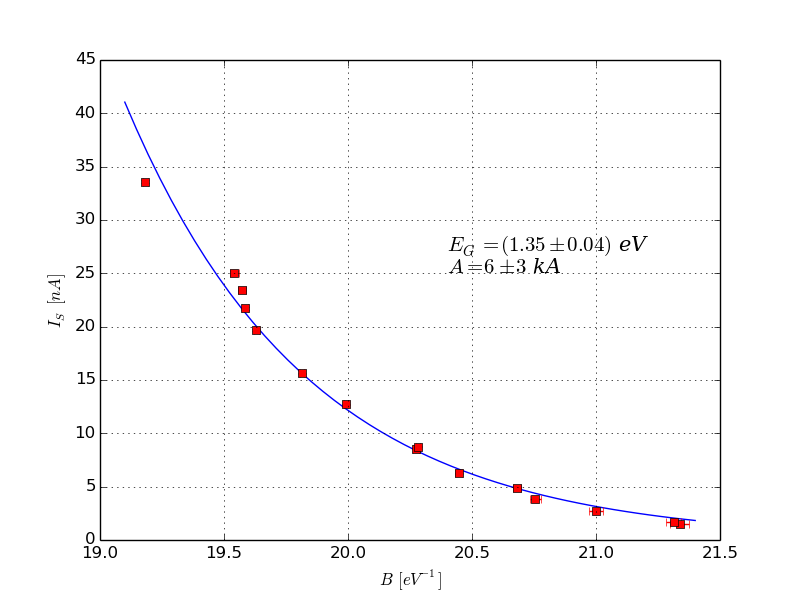
\includegraphics[scale=.5]{fit_eg}
\caption{Best fit per l'energy gap}
\label{fig:fiteg}
\end{figure}

\begin{table}[!h]
\centering
\caption{Risultati del fit}
\label{tab:fit}
\begin{tabular}{|c|c|} 
\hline 
$E_G$ & 1.35(4) eV \\ 
\hline 
A & 6(3) kA \\ 
\hline 
$\chi ^2$/ndof & 4953 \\ 
\hline 
Corr. & 0.9997 \\ 
\hline 
\end{tabular} 
\end{table}

Come si vede i parametri sono estremamente correlati, per cui variando poco il valore di $E_G$ la stima di A cambia anche di ordini di grandezza. Per quanto riguarda il valore di $E_G$, non è compatibile con quello atteso per il diodo in esame, circa 1.12 eV, questo a causa delle problematiche del fit.\\
È stato stimato il valore dell'energy gap anche tenendo conto del fatto che il valore di $\delta$ è diverso da 0. In questo caso si è proceduto iterativamente attraverso l'equazione \ref{eqn:schock} manipolata come segue:

\begin{equation}
I_S = A \exp (\delta \log T - BE_G) = A \exp \Bigg (E_G \bigg (\frac{\delta}{E_G} \log T - B \bigg ) \Bigg )
\end{equation}

Il metodo è stato inserire per il primo step un valore iniziale per $E_G$ al denominatore, dopodiché effettuare un fit a due parametri per ottenere una stima successiva dell'energy gap, procedendo poi iterativamente. I risultati sono mostrati, per $\delta$ = 1.5 e $\delta$ = 2, in figure \ref{fig:tiger} e  \ref{fig:mouse}.

\begin{figure}[!h]
\centering
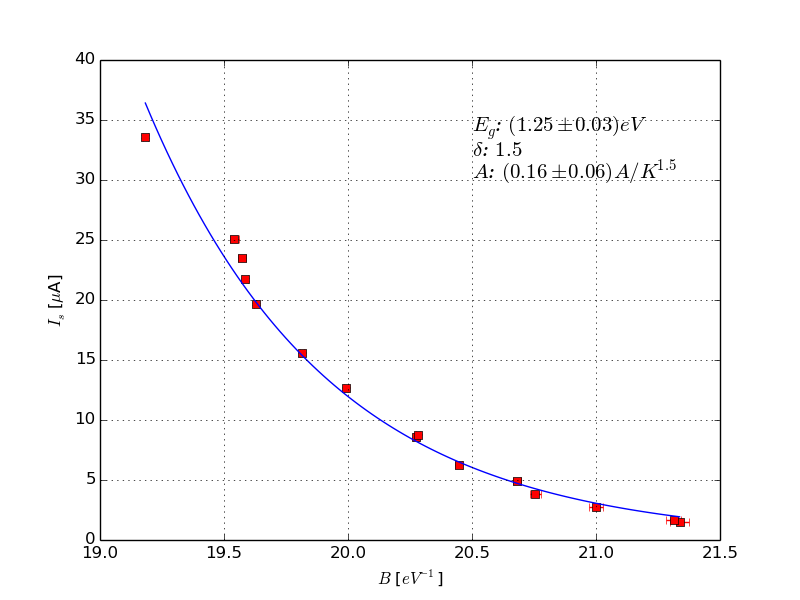
\includegraphics[scale=.5]{energygap_first_recursive1-5}
\caption{Best fit ricorsivo, $\delta$ = 1.5}
\label{fig:tiger}
\end{figure}
   
\begin{figure}[!h]
\centering
        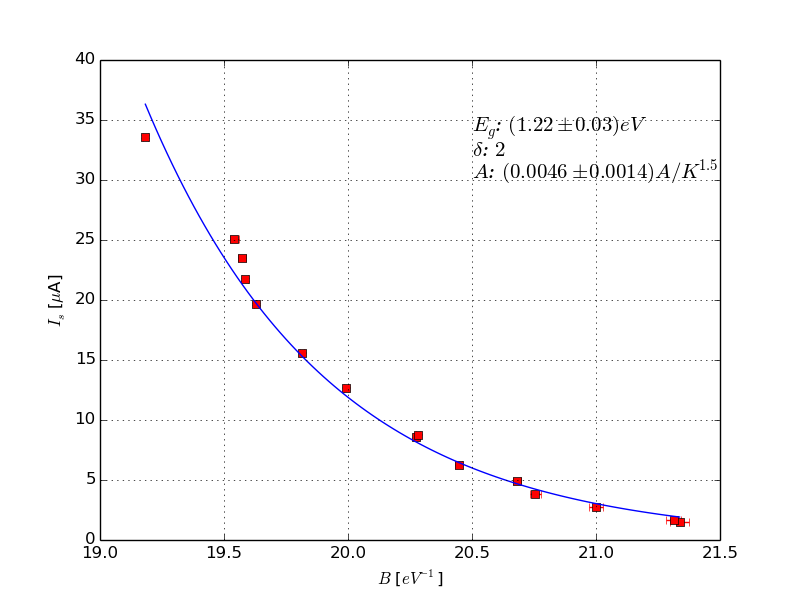
\includegraphics[scale=.5]{energygap_first_recursive2}
        \caption{Best fit ricorsivo, $\delta$ = 2}
        \label{fig:mouse}
\end{figure}

\subsection{Determinazione a partire dai dati V-T}

Un altro metodo per stimare l'energy gap del diodo consiste nel fissare un valore della corrente in cui la curva caratteristica segue l'andamento esponenziale alla Shockley e valutare l'andamento della tensione in funzione della temperatura interpolando i dati. Una volta ottenuti i dati di T in funzione di V, a partire dall'equazione di Shockley:

\begin{equation}
I = I_A \exp \frac{V_eE_G}{nkT}
\end{equation}

si ottiene:

\begin{equation}
\label{eqn:lin}
T = aV +b
\end{equation}

con:

\begin{gather}
a = -\frac{1}{nk \log \frac{I_A}{I}} \\
b = \frac{eE_G}{nk \log \frac{I_A}{I}}
\end{gather}

da cui facendo un best fit a partire dalla \ref{eqn:lin}, si ricavano i valori di \emph{a} e \emph{b} e da questi quello di $E_G$:

\begin{equation}
E_G = \frac{b}{a}
\end{equation}

I risultati sono mostrati in figura \ref{fig:int}.

\begin{figure}[!h]
\centering
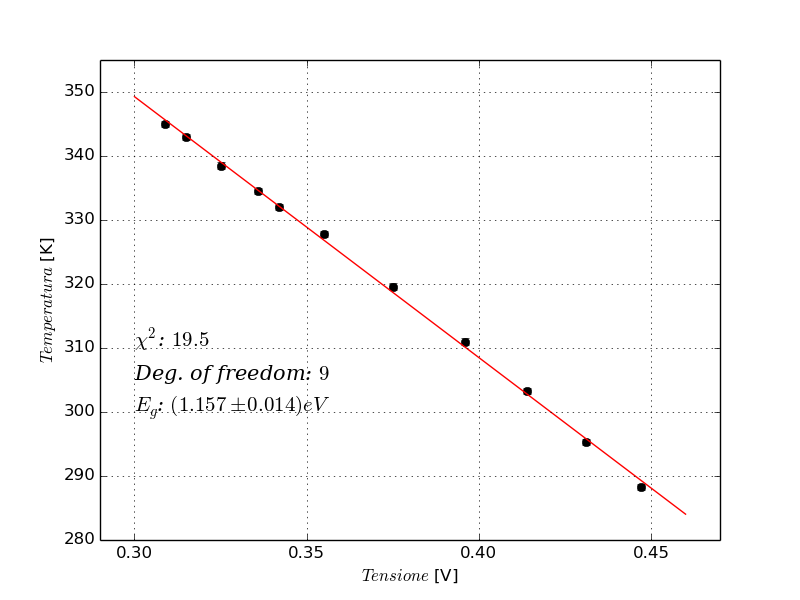
\includegraphics[scale=.5]{interpol}
\caption{Fit dei dati interpolati}
\label{fig:int}
\end{figure}

L'energy gap è più ragionevole, benché ancora significativamente più alto di quello atteso, e il $\chi ^2$ buono, per cui in questo caso quest'ultimo metodo si è rivelato più efficace.

\end{itemize}
\begin{thebibliography}{10}
\bibitem{bib1}
Lorem M, Ipsum VE (1990) Rank Correlation Methods. New York: Oxford University Press, 5th edition.

\bibitem{bib2}
Ipsum M, Ipsum JD (1990) Rank Correlation Methods. New York: Oxford University Press, 5th edition.

\end{thebibliography}



\end{document}